\documentclass[sigconf,nonacm]{acmart}

\makeatletter
\def\@ACM@checkaffil{}
\makeatother

\settopmatter{printacmref=false}
\setcopyright{cc}
\setcctype{by-sa}

\newcommand\mycommfont[1]{\footnotesize\ttfamily\textcolor{gray}{#1}}

% defining the \BibTeX command - from Oren Patashnik's original BibTeX documentation.
\def\BibTeX{{\rm B\kern-.05em{\sc i\kern-.025em b}\kern-.08emT\kern-.1667em\lower.7ex\hbox{E}\kern-.125emX}}
    
\usepackage{nicefrac}
\usepackage{siunitx}
\usepackage{array,framed}
\usepackage{booktabs}
\usepackage{
  color,
  float,
  epsfig,
  wrapfig,
  graphics,
  graphicx,
  subcaption
}

\usepackage{textcomp,amssymb}
\usepackage{setspace}
\usepackage{latexsym,fancyhdr,url}
\usepackage{enumerate}
\usepackage{algorithm2e}
\usepackage{algpseudocode}
\usepackage{graphics}
\usepackage{xparse} % argument parsing -- \edist
\usepackage{xspace}
\usepackage{multirow}
\usepackage{csvsimple}
\usepackage{balance}

\usepackage{
  tikz,
  pgfplots,
  pgfplotstable
}
\usepackage{hyperref}

\usetikzlibrary{
  shapes.geometric,
  arrows,
  external,
  pgfplots.groupplots,
  matrix
}

\pgfplotsset{compat=1.9}

\usepackage{mathtools,}
\DeclarePairedDelimiter\abs{\lvert}{\rvert}
\DeclarePairedDelimiter\norm{\lVert}{\rVert}

\DeclareMathAlphabet{\mathcal}{OMS}{cmsy}{m}{n}

\DeclareGraphicsExtensions{%
    .png,.PNG,%
    .pdf,.PDF,%
    .jpg,.mps,.jpeg,.jbig2,.jb2,.JPG,.JPEG,.JBIG2,.JB2}

\usepackage{xparse}
\newcommand{\bnm}{\begin{newmath}}
\newcommand{\enm}{\end{newmath}}

\newcommand{\bea}{\begin{eqnarray*}}%
\newcommand{\eea}{\end{eqnarray*}}%

\newcommand{\bne}{\begin{newequation}}
\newcommand{\ene}{\end{newequation}}

\newcommand{\bal}{\begin{newalign}}
\newcommand{\eal}{\end{newalign}}

\newenvironment{newalign}{\begin{align}%
\setlength{\abovedisplayskip}{4pt}%
\setlength{\belowdisplayskip}{4pt}%
\setlength{\abovedisplayshortskip}{6pt}%
\setlength{\belowdisplayshortskip}{6pt} }{\end{align}}

\newenvironment{newmath}{\begin{displaymath}%
\setlength{\abovedisplayskip}{4pt}%
\setlength{\belowdisplayskip}{4pt}%
\setlength{\abovedisplayshortskip}{6pt}%
\setlength{\belowdisplayshortskip}{6pt} }{\end{displaymath}}

\newenvironment{neweqnarrays}{\begin{eqnarray*}%
\setlength{\abovedisplayskip}{-4pt}%
\setlength{\belowdisplayskip}{-4pt}%
\setlength{\abovedisplayshortskip}{-4pt}%
\setlength{\belowdisplayshortskip}{-4pt}%
\setlength{\jot}{-0.4in} }{\end{eqnarray*}}

\newenvironment{newequation}{\begin{equation}%
\setlength{\abovedisplayskip}{4pt}%
\setlength{\belowdisplayskip}{4pt}%
\setlength{\abovedisplayshortskip}{6pt}%
\setlength{\belowdisplayshortskip}{6pt} }{\end{equation}}


\newcounter{ctr}
\newcounter{savectr}
\newcounter{ectr}

\newenvironment{newitemize}{%
\begin{list}{\mbox{}\hspace{5pt}$\bullet$\hfill}{\labelwidth=15pt%
\labelsep=4pt \leftmargin=12pt \topsep=3pt%
\setlength{\listparindent}{\saveparindent}%
\setlength{\parsep}{\saveparskip}%
\setlength{\itemsep}{3pt} }}{\end{list}}


\newenvironment{newenum}{%
\begin{list}{{\rm (\arabic{ctr})}\hfill}{\usecounter{ctr} \labelwidth=17pt%
\labelsep=5pt \leftmargin=22pt \topsep=3pt%
\setlength{\listparindent}{\saveparindent}%
\setlength{\parsep}{\saveparskip}%
\setlength{\itemsep}{2pt} }}{\end{list}}

%%%%%%%%%%%%%%%%%%%%%%%%%%%%%%%%%%%%%%%%%%%%%%%%%%%%%%%%%%%%%%%%%%%%%%%%%%%%%%
%
% Figure and table macros
%

\newcounter{mytable}
\def\mytable{\begin{centering}\refstepcounter{mytable}}
\def\endmytable{\end{centering}}

\def\mytablecaption#1{\vspace{2mm}
  \centerline{Table \arabic{mytable}.~{#1}}
  \vspace{6mm}
  \addcontentsline{lot}{table}{\protect\numberline{\arabic{mytable}}~{#1}}
}


\newcounter{myfig}
\def\myfig{\begin{centering}\refstepcounter{myfig}}
\def\endmyfig{\end{centering}}

\def\myfigcaption#1{
             \vspace{2mm}
             \centerline{\textsf{Figure \arabic{myfig}.~{#1}}}
             \vspace{6mm}
             \addcontentsline{lof}{figure}{\protect\numberline{\arabic{myfig}}~{#1}}}


\newlength{\saveparindent}
\setlength{\saveparindent}{\parindent}
\newlength{\saveparskip}
\setlength{\saveparskip}{\parskip}

\newcommand{\decOracle}{\textbf{Dec}}

\newcommand{\negsmidge}{{\hspace{-0.1ex}}}
\newcommand{\cdotsm}{\negsmidge\negsmidge\negsmidge\cdot\negsmidge\negsmidge\negsmidge}

\def\suchthatt{\: :\:}
\newcommand{\E}{{\rm I\kern-.3em E}}
\newcommand{\Prob}[1]{{\Pr\left[\,{#1}\,\right]}}
\newcommand{\Probb}[2]{{\Pr}_{#1}\left[\,{#2}\,\right]}
\newcommand{\CondProb}[2]{{\Pr}\left[\: #1\:\left|\right.\:#2\:\right]}
\newcommand{\CondProbb}[2]{\Pr[#1|#2]}
\newcommand{\ProbExp}[2]{{\Pr}\left[\: #1\:\suchthatt\:#2\:\right]}
\newcommand{\Ex}[1]{{\textnormal{E}\left[\,{#1}\,\right]}}
\newcommand{\Exx}{{\textnormal{E}}}
\newcommand{\given}{\ensuremath{\,\big|\,}}


\newcommand{\true}{\mathsf{true}}
\newcommand{\false}{\mathsf{false}}
\def\negl{\mathsf{negl}}


\newcommand{\secref}[1]{\mbox{Section~\ref{#1}}}
\newcommand{\appref}[1]{\mbox{Appendix~\ref{#1}}}
\newcommand{\thref}[1]{\mbox{Theorem~\ref{#1}}}
\newcommand{\defref}[1]{\mbox{Definition~\ref{#1}}}
\newcommand{\corref}[1]{\mbox{Corollary~\ref{#1}}}
\newcommand{\lemref}[1]{\mbox{Lemma~\ref{#1}}}
\newcommand{\clref}[1]{\mbox{Claim~\ref{#1}}}
\newcommand{\propref}[1]{\mbox{Proposition~\ref{#1}}}
\newcommand{\factref}[1]{\mbox{Fact~\ref{#1}}}
\newcommand{\remref}[1]{\mbox{Remark~\ref{#1}}}
\newcommand{\figref}[1]{\mbox{Figure~\ref{#1}}}
\renewcommand{\algref}[1]{\mbox{Algorithm~\ref{#1}}}
% \newcommand{\eqref}[1]{\mbox{Equation~(\ref{#1})}}
% Have to use \renewcommand because exists already in amsmath
\renewcommand{\eqref}[1]{\mbox{Equation~(\ref{#1})}}
\newcommand{\consref}[1]{\mbox{Construction~\ref{#1}}}
\newcommand{\tabref}[1]{\mbox{Table~\ref{#1}}}

\newcommand{\get}{{\:{\leftarrow}\:}}
\newcommand{\gett}[1]{\:{\leftarrow}_{#1}\:}
\newcommand{\getsr}{{\:{\leftarrow{\hspace*{-3pt}\raisebox{.75pt}{$\scriptscriptstyle\$$}}}\:}}
\newcommand{\getm}{{\:\leftarrow_{\mdist}\:}}
\newcommand{\getd}{{\:\leftarrow_{\ddist}\:}}
%\newcommand{\getm}{{\:{\leftarrow{\hspace*{-3pt}\raisebox{.75pt}{$\scriptscriptstyle \mdist$}}}\:}}
\newcommand{\getk}{{\:\leftarrow_{\kdist}\:}}
%\newcommand{\getk}{{\:{\leftarrow{\hspace*{-3pt}\raisebox{.75pt}{$\scriptscriptstyle \kdist$}}}\:}}
\newcommand{\getp}{{\:\leftarrow_{p}\:}}



\newcommand{\gamesfontsize}{\small}
\newcommand{\fpage}[2]{\framebox{\begin{minipage}[t]{#1\textwidth}\setstretch{1.1}\gamesfontsize  #2 \end{minipage}}}
\newcommand{\mpage}[2]{\begin{minipage}[t]{#1\textwidth}\setstretch{1.1}\gamesfontsize  #2 \end{minipage}}

\newcommand{\hpages}[3]{\begin{tabular}{cc}\begin{minipage}[t]{#1\textwidth} #2 \end{minipage} & \begin{minipage}[t]{#1\textwidth} #3 \end{minipage}\end{tabular}}

\newcommand{\hpagess}[4]{
        \begin{tabular}[t]{c@{\hspace*{.5em}}c}
        \begin{minipage}[t]{#1\textwidth}\gamesfontsize #3 \end{minipage}
        &
        \begin{minipage}[t]{#2\textwidth}\gamesfontsize #4 \end{minipage}
        \end{tabular}
    }

\newcommand{\hpagesss}[6]{
        \begin{tabular}[t]{c@{\hspace*{.5em}}c@{\hspace*{.5em}}c@{\hspace*{.5em}}c}
        \begin{minipage}[t]{#1\textwidth}\gamesfontsize #4 \end{minipage}
        &
        \begin{minipage}[t]{#2\textwidth}\gamesfontsize #5 \end{minipage}
        &
        \begin{minipage}[t]{#3\textwidth}\gamesfontsize #6 \end{minipage}
        \end{tabular}
    }

\newcommand{\hpagessss}[8]{
        \begin{tabular}{c@{\hspace*{.5em}}c@{\hspace*{.5em}}c@{\hspace*{.5em}}c}
        \begin{minipage}[t]{#1\textwidth}\gamesfontsize #5 \end{minipage}
        &
        \begin{minipage}[t]{#2\textwidth}\gamesfontsize #6 \end{minipage}
        &
        \begin{minipage}[t]{#3\textwidth}\gamesfontsize #7 \end{minipage}
        &
        \begin{minipage}[t]{#4\textwidth}\gamesfontsize #8 \end{minipage}
        \end{tabular}
    }


\newcommand{\hfpages}[3]{\hfpagess{#1}{#1}{#2}{#3}}
\newcommand{\hfpagess}[4]{
        \begin{tabular}[t]{c@{\hspace*{.5em}}c}
        \framebox{\begin{minipage}[t]{#1\textwidth}\setstretch{1.1}\gamesfontsize #3 \end{minipage}}
        &
        \framebox{\begin{minipage}[t]{#2\textwidth}\setstretch{1.1}\gamesfontsize #4 \end{minipage}}
        \end{tabular}
    }
\newcommand{\hfpagesss}[6]{
        \begin{tabular}[t]{c@{\hspace*{.5em}}c@{\hspace*{.5em}}c}
        \framebox{\begin{minipage}[t]{#1\textwidth}\setstretch{1.1}\gamesfontsize #4 \end{minipage}}
        &
        \framebox{\begin{minipage}[t]{#2\textwidth}\setstretch{1.1}\gamesfontsize #5 \end{minipage}}
        &
        \framebox{\begin{minipage}[t]{#3\textwidth}\setstretch{1.1}\gamesfontsize #6 \end{minipage}}
        \end{tabular}
    }
\newcommand{\hfpagessss}[8]{
        \begin{tabular}[t]{c@{\hspace*{.5em}}c@{\hspace*{.5em}}c@{\hspace*{.5em}}c}
        \framebox{\begin{minipage}[t]{#1\textwidth}\setstretch{1.1}\gamesfontsize #5 \end{minipage}}
        &
        \framebox{\begin{minipage}[t]{#2\textwidth}\setstretch{1.1}\gamesfontsize #6 \end{minipage}}
        &
        \framebox{\begin{minipage}[t]{#3\textwidth}\setstretch{1.1}\gamesfontsize #7 \end{minipage}}
        &
        \framebox{\begin{minipage}[t]{#4\textwidth}\setstretch{1.1}\gamesfontsize #8 \end{minipage}}
        \end{tabular}
    }

\newcommand{\vecw}{\mathbf{w}}
\newcommand{\R}{\mathbb{R}}
\newcommand{\N}{\mathbb{N}}
\newcommand{\Z}{\mathbb{Z}}
\newcommand{\load}{L}
\newcommand{\coll}{\mathsf{Coll}}
\newcommand{\nocoll}{\overline{\mathsf{Coll}}}


\newcommand{\Img}{\textsf{Img}}

%%%%%%%%%%%%%%%%%%%%%%%%%%%%%%%%%%%%%%%%%%%%%%%%%%%%%%%%%%%%%%%%%%%%%%%%%%%%%%%%
%%%% Fonts and symbols
%%%%%%%%%%%%%%%%%%%%%%%%%%%%%%%%%%%%%%%%%%%%%%%%%%%%%%%%%%%%%%%%%%%%%%%%%%%%%%%%
\newcommand\funcfont{\textsf}
\newcommand\variablefont{\texttt}

%%%%%%%%%%%%%%%%%%%%%%%%%%%%%%%%%%%%%%%%%%%%%%%%%%%%%%%%%%%%%%%%%%%%%%%%%%%%%%%%
%%%%%%%%%%%%%%%%%%%%%%%%%%%%%%%% NEW COMMANDS %%%%%%%%%%%%%%%%%%%%%%%%%%%%%%%%%%
%%%%%%%%%%%%%%%%%%%%%%%%%%%%%%%%%%%%%%%%%%%%%%%%%%%%%%%%%%%%%%%%%%%%%%%%%%%%%%%%

\def \Perm {\funcfont{Perm}}
\def \calC {{\mathcal{C}}}
\def \calU {{\mathcal{U}}}
\renewcommand{\u}{\ensuremath{u}}
\newcommand{\unew}{\ensuremath{\tilde{u}}}

\newcommand{\calN}{\mathcal{N}}
\def \sspace {{\mathcal{S}}}
\def \strings {{\mathcal{S}}}
\def \slen {{s}}
\def \kspace {{\mathcal{K}}}
\def \kspacesize {{m}}
\def \mspacesize {{n}}
\def \kdict {D}
\def \dictsize {d}
\newcommand{\kdist}{p_k}
\newcommand{\mdist}{\ensuremath{{W}}}
\newcommand{\alldist}{\rho}
\newcommand{\pwdist}{\transgen}
\newcommand{\ddist}{\rho_{dec}}
\newcommand{\PWset}{{\mathcal{P}}}  % TODO: fix, same as \pwdist
\newcommand{\PWsetvec}{\vec{\mathcal{P}}}
\newcommand{\PWvec}{\vec{P}}
\newcommand{\domvec}{\vec{D}}
\newcommand{\humanornot}{\vec{h}}
\newcommand{\dom}{\textsf{dom}}
%\def \kdist {{\kappa}}
%\def \mdist {{\mu}}
%\def \ddist {{\delta}}
\def \pspace {{\mathcal{P}}}
\def \mpspace {{\mathcal{MP}}}
\def \cspace {{\mathcal{C}}}
\def \key {\kappa}
\def \msg {M}
\def \seed {S}
\def \ctxt {C}
\def \ctxtpart {C_2}
\newcommand{\genprime}{{\textsf{GenPrime}}}
\newcommand{\isprime}{{\textsf{IsPrime}}}
\newcommand{\LeastLesserPrime}{{\textsf{PrevPrime}}}
\newcommand{\pwset}{\mathcal{S}}
\newcommand{\DTE}{{\textsf{DTE}}}
\newcommand{\encode}{{\textsf{encode}}}
\newcommand{\decode}{{\textsf{decode}}}

\newcommand{\DTEsingle}{{\textsf{1PW-DTE}}}
\newcommand{\encodesingle}{{\textsf{1PW-encode}}}
\newcommand{\decodesingle}{{\textsf{1PW-decode}}}

\newcommand{\DTErss}{{\textsf{RSS-DTE}}}
\newcommand{\encoderss}{{\textsf{RSS-encode}}}
\newcommand{\decoderss}{{\textsf{RSS-decode}}}

\newcommand{\DTEindep}{{\textsf{MPW-DTE}}}
\newcommand{\encodeindep}{{\textsf{MPW-encode}}}
\newcommand{\decodeindep}{{\textsf{MPW-decode}}}


\newcommand{\DTEsub}{{\textsf{SG-DTE}}}
\newcommand{\encodesub}{{\textsf{SG-encode}}}
\newcommand{\decodesub}{{\textsf{SG-decode}}}
\newcommand{\decodekamf}{{\textsf{KAMF-decode}}}
\newcommand{\DTEis}{{\textsf{IS-DTE}}}
\newcommand{\encodeis}{{\textsf{is-encode}}}
\newcommand{\decodeis}{{\textsf{is-decode}}}
\newcommand{\DTErej}{{\textsf{REJ-DTE}}}
\newcommand{\encoderej}{{\textsf{rej-encode}}}
\newcommand{\decoderej}{{\textsf{rej-decode}}}
\newcommand{\DTErsarej}{{\textsf{RSA-REJ-DTE}}}
\newcommand{\encodeRSAREJ}{{\textsf{rsa-rej-encode}}}
\newcommand{\decodeRSAREJ}{{\textsf{rsa-rej-decode}}}
\newcommand{\DTErsainc}{{\textsf{RSA-INC-DTE}}}
\newcommand{\encodeRSAINC}{{\textsf{rsa-inc-encode}}}
\newcommand{\decodeRSAINC}{{\textsf{rsa-inc-decode}}}
\newcommand{\DTEunf}{{\textsf{UNF-DTE}}}
\newcommand{\DTEnunf}{{\textsf{NUNF-DTE}}}


%\newcommand{\encodeis}{{\textsf{encode}_{\textrm{is}}}}
%\newcommand{\decodeis}{{\textsf{decode}_{\textrm{is}}}}
\newcommand{\rep}{\textsf{rep}}
\newcommand{\isErr}{\epsilon_{\textnormal{is}}}
\newcommand{\incErr}{\epsilon_{\textnormal{inc}}}
\def \enc {{\textsf{E}}}
\def \dec {{\textsf{D}}}
\def \SEscheme {{\textsf{SE}}}
\def \HEscheme {{\textsf{HE}}}
\def \CTR {{\textsf{CTR}}}
\def \encHE {{\textsf{HEnc}}}
\def \HIDE {{\textsf{HiaL}}}
\def \encHIDE {{\textsf{HEnc}}}
\def \decHIDE {{\textsf{HDec}}}
\def \decHE {{\textsf{HDec}}}
\def \encHEt {{\textsf{HEnc2}}}
\def \decHEt {{\textsf{HDec2}}}

\newcommand{\myind}{\hspace*{1em}}
\newcommand{\thh}{^{\textit{th}}} % th
\newcommand{\concat}{\,\|\,}
\newcommand{\dotdot}{..}
\newcommand{\emptystr}{\varepsilon}

\newcommand{\round}{\textsf{round}}

\newcommand{\alphabar}{\overline{\alpha}}
\newcommand{\numbinsbar}{\overline{b}}
\newcommand{\numballs}{a}
\newcommand{\numbins}{b}

%\def \encHE {{\sf{enc}^{HE}}}
%\def \decHE {{\sf{dec}^{HE}}}
%\def \encHEt {{\sf{enc}^{HE2}}}
%\def \decHEt {{\sf{dec}^{HE2}}}
\def \idealHE {{\mathcal{HE}}}
\def \IEnc {{\mathbf{\rho}}}
\def \IDec {{\mathbf{\rho^{-1}}}}
\def \OEnc {{\mathbf{Enc}}}
\def \ODec {{\mathbf{Dec}}}
\newcommand{\SimuProc}{\mathbf{Sim}}
\newcommand{\ROProc}{\mathbf{RO}}
\newcommand{\PrimProc}{\mathbf{Prim}}
\def \stm {g}
\def \istm {\hat{g}}
\def \kts {{f}}
\def \lex {{\sf lex}}
\def \part {part}
\def \kd {{\sf{kd}}}
\def \msgdist {{d}}
\def \keydist {{r}}
\def \ind {{\sf{index}}}
\def \kprf {z}
\def \adv {{\mathcal A}}
\def \pwds {u}
\newcommand{\mpw}{mpw}
\newcommand{\pw}{w}
\newcommand{\pwvec}{\vec{\pw}}
\newcommand{\vecx}{\vec{x}}
\def \tokens {v}
\def \calP{{\mathcal{P}}}
\def \template{{\mathcal{T}}}
\def \vaultset{{\mathcal{V}}}
\def \ext {{\sf ext}}
\def \offset {\delta}
\def \maxweight {\epsilon}
\def \advo {{\mathcal{A}}^{*}}

\newcommand{\Chall}{\textsf{Ch}}
\newcommand{\Test}{\textnormal{\textsf{Test}}}
\newcommand{\RoR}{\textsf{RoR}}
\newcommand{\MI}{\textnormal{MI}}
\providecommand{\MR}{\textnormal{MR}}
\newcommand{\MRCCA}{\textnormal{MR-CCA}}
\newcommand{\SAMP}{\textnormal{SAMP}}
\newcommand{\DTEgame}{\textnormal{SAMP}}
\newcommand{\KR}{\textnormal{KR}}
\newcommand{\advA}{{\mathcal{A}}}
\newcommand{\advR}{{\mathcal{R}}}
\newcommand{\advB}{{\mathcal{B}}} % 
\newcommand{\advC}{{\mathcal{C}}} % C
\newcommand{\advD}{{\mathcal{D}}} % D
\newcommand{\advE}{{\mathcal{E}}}
\newcommand{\advF}{{\mathcal{F}}}
\newcommand{\advG}{{\mathcal{G}}}
\newcommand{\advI}{{\mathcal{I}}}
\newcommand{\nextval}{\;;\;}
\newcommand{\TabC}{\texttt{C}}
\newcommand{\TabR}{\texttt{R}}
\newcommand{\Hash}{H}
\newcommand{\Cipher}{\pi}
\newcommand{\CipherInv}{\pi^{-1}}
\newcommand{\simu}{{\mathcal S}}
\newcommand{\prim}{P}
\newcommand{\maxguess}{\gamma}


\newcommand{\bigO}{\mathcal{O}}
\newcommand{\calG}{{\mathcal{G}}}

\def\sqed{{\hspace{5pt}\rule[-1pt]{3pt}{9pt}}}
\def\qedsym{\hspace{2pt}\rule[-1pt]{3pt}{9pt}}

\newcommand{\Colon}{{\::\;}}
\newcommand{\good}{\textsf{Good}}

\newcommand\Tvsp{\rule{0pt}{2.6ex}}
\newcommand\Bvsp{\rule[-1.2ex]{0pt}{0pt}}
\newcommand{\TabPad}{\hspace*{5pt}}
\newcommand\TabSep{@{\hspace{5pt}}|@{\hspace{5pt}}}
\newcommand\TabSepLeft{|@{\hspace{5pt}}}
\newcommand\TabSepRight{@{\hspace{5pt}}|}


\DeclareMathOperator*{\argmin}{argmin}
\DeclareMathOperator*{\argmax}{argmax}
\newcommand{\comma}{\textnormal{,}}

\renewcommand{\paragraph}[1]{\vspace*{6pt}\noindent\textbf{#1}\;}

\newcommand{\weirvault}{\textsf{Pastebin}\xspace}
\newcommand{\ndssvault}{\textsf{DBCBW}\xspace}




\newcommand{\reminder}[1]{ [[[ \marginpar{\mbox{$<==$}} #1 ]]] }

%
% New theorem types: (Already in CCS template)
%
\newtheorem{observation}{Observation}
%\newtheorem{definition}{Definition}
\newtheorem{claim}{Claim}
\newtheorem{assumption}{Assumption}
\newtheorem{fact}{Fact}
% \newtheorem{theorem}{Theorem}[section]
% \newtheorem{lemma}{Lemma}[section]
% \newtheorem{corollary}{Corollary}[section]
% \newtheorem{proposition}{Proposition}
% \newtheorem{example}{Example}

%
% Definitions:
%
\def \blackslug{\hbox{\hskip 1pt \vrule width 4pt height 8pt
    depth 1.5pt \hskip 1pt}}
\def \qed{\quad\blackslug\lower 8.5pt\null\par}
% In-line QED, for ending a proof with a $$ formula
% In-line QED, for ending a proof with a $$ formula
\def \inQED{\quad\quad\blackslug}
\def \Qed{\QED}
\def \QUAD{$\Box$}
\def \Proof{\par\noindent{\bf Proof:~}}
\def \proof{\Proof}
\def \poly {\mbox{$\mathsf{poly}$}}
\def \binary {\mbox{$\mathsf{binary}$}}
\def \ones {\mbox{$\mathsf{ones}$}}
\def \rank {\mbox{$\mathsf{rank}$}}
\def \bits {\mbox{$\mathsf{bits}$}}
\def \factorial {\mbox{$\mathsf{factorial}$}}
\def \fr {\mbox{$\mathsf{fr}$}}
\def \pr {\mbox{$\mathsf{pr}$}}
\def \zon {\{0,1\}^n}
\def \zo  {\{0,1\}}
\def \zok {\{0,1\}^k}
\def \mo {s}


\def\utilcnt{\ensuremath{\mu_{\mathrm{cnt}}}}
\def\utiltime{\ensuremath{\mu_{\mathrm{time}}}}
\def\ex{\ensuremath{{\mathrm{ex}}}}
\def\rlx{\ensuremath{{\mathrm{rlx}}}}
\def\tp{\textsf{TP}}
\def\cp{\textnormal{\textsf{CP}}\xspace}
\def\edistcutoff{\edist}
\def\entcutoff{\ensuremath{m}}
\def\relentcutoff{{\sigma}}
\def\mutt{\mu_{\mathrm{tt}}}

\newcommand{\Hdot}{H(\mbox{ } \cdot \mbox{ }  , \mbox{ } \del)}


\newcounter{mynote}[section]
\newcommand{\notecolor}{blue}
\newcommand{\thenote}{\thesection.\arabic{mynote}}
\newcommand{\tnote}[1]{\refstepcounter{mynote}{\bf \textcolor{\notecolor}{$\ll$TomR~\thenote: {\sf #1}$\gg$}}}

\newcommand{\fixme}[1]{{\textcolor{red}{[FIXME: #1]}}}
\newcommand{\todo}[1]{{\textcolor{red}{[TODO: #1]}}}


\newcommand\ignore[1]{}


\newcommand\simplescheme{simple}


\newcommand{\KDF}{\mathsf{KDF}}
\newcommand{\salt}{\mathsf{sa}}
\newcommand{\PRF}{F}
\newcommand{\subgram}{\mathsf{SG}}
\newcommand{\popdomains}{\mathcal{D}}

\newcommand{\retrieve}{\textsf{Sync}}
\newcommand{\update}{\textsf{Insert}}

\newcommand{\dictW}{\textbf{D1}\xspace}
\newcommand{\dictF}{\textbf{D2}\xspace}

\newcommand{\str}{\text{str}}
\newcommand{\calS}{{\mathcal S}}

% \newcommand{\new}[1]{\textcolor{red}{\sf #1}}
\newcommand{\new}[1]{#1}


%% ------------------------- Rahul -----------------------
\newcounter{rcnote}[section]
\newcommand{\rcthenote}{\thesection.\arabic{rcnote}}
\newcommand{\rcnote}[1]{\refstepcounter{rcnote}{\bf \textcolor{magenta}{$\ll$RC~\rcthenote: {\sf #1}$\gg$}}}

\newcounter{mrnote}[section]
\newcommand{\mrthenote}{\thesection.\arabic{mrnote}}
\newcommand{\mrnote}[1]{\refstepcounter{mrnote}{\bf \textcolor{green}{$\ll$MR~\mrthenote: {\sf #1}$\gg$}}}

\newcounter{fknote}[section]
\newcommand{\fkthenote}{\thesection.\arabic{fknote}}
\newcommand{\fknote}[1]{\refstepcounter{fknote}{\bf \textcolor{blue}{$\ll$FK~\fkthenote: {\sf #1}$\gg$}}}

\newcounter{anote}[section]
\newcommand{\ajthenote}{\thesection.\arabic{anote}}
\newcommand{\anote}[1]{\refstepcounter{anote}{\bf \textcolor{cyan}{$\ll$AJ~\ajthenote: {\sf #1}$\gg$}}}



\newcommand{\mytab}{\hspace*{.4cm}}
\def\half{{1\over 2}}
\newcommand{\NT}[1]{\texttt{#1}}
\DeclareMathSymbol{\mlq}{\mathord}{operators}{``}
\DeclareMathSymbol{\mrq}{\mathord}{operators}{`'}
\newcommand{\calO}{{\mathcal O}}
\newcommand{\calA}{{\mathcal A}}
\newcommand{\kamfplus}{Kamouflage\textbf{+}\xspace}
% \newcommand{\genfrom}[1]{\;{\stackrel{\,#1}{\leftarrow}}\;}
\newcommand{\genfrom}[1]{{\:{\leftarrow{\hspace*{-3pt}\raisebox{.75pt}{$\scriptscriptstyle#1$}}}\:}}
%\newcommand{\genfrom}[1]{\;\leftarrow{\tiny \$} #1\;}
\newcommand{\twopartdef}[4]
{
  \left\{
    \begin{array}{ll}
      #1 & \mbox{if } #2 \\[4pt]
      #3 & #4
      \end{array}
      \right.
}
\newcommand{\threepartdef}[6]
{
  \left\{
    \begin{array}{lll}
      #1 & \mbox{if } #2 \\
      #3 & \mbox{if } #4 \\
      #5 & \mbox{if } #6
      \end{array}
      \right.
}

\newcommand{\gt}[1]{\gamma_{#1,\maxdist}}
\newcommand{\gmt}[2]{\gamma_{#1,#2}}
\def\nh{\ensuremath{N}}
\def\ball{\ensuremath{B}}
\def\anh{\ensuremath{\tilde{N}_k}}
% \newcommand{\nh}[2]{{N_{#1}(#2)}}

\newcommand{\ballsizet}[1]{{\beta_{#1,\maxdist}}}
\newcommand{\ballsize}[2]{{\beta_{#1,#2}}}
\newcommand{\rh}[2]{{\bf R}_{#1, #2}}
\newcommand{\rhf}[2]{R_{f, \gamma}}
\newcommand{\realm}{{m}}
% \newcommand{\inputm}{{\tilde{m}}}
\newcommand{\lmid}{\ell_{\realm, m'}}
\newcommand{\cipherlength}{n}
\renewcommand{\SS}{\textsf{SS}}
\newcommand{\Rec}{\textsf{Rec}\xspace}
\newcommand{\rec}{\textsf{rec}\xspace}
\newcommand{\Rep}{\textsf{Rep}\xspace}
\newcommand{\Gen}{\textsf{Gen}}
\newcommand{\dis}{\textsf{dis}}

\def\chk{\textnormal{\textsf{Chk}}\xspace}
\def\reg{\textnormal{\textsf{Reg}}\xspace}
\def\exchk{\textnormal{\textsf{ExChk}}\xspace}
\def\adpchk{\textnormal{\textsf{AdpChk}}\xspace}
\def\RKROR{\textnormal{MKROR}\xspace}
\def\SRKROR{\textnormal{SKROR}\xspace}
\def\ROR{\textnormal{ROR}\xspace}
\def\ROBUST{\textnormal{ROB}\xspace}
\def\OFFDIST{\textnormal{OFFDIST}\xspace}
\def\POFFDIST{\overline{\textnormal{OFFDIST}}\xspace}
\def\OFFGUESS{\textnormal{OFFGUESS}\xspace}
\def\ONGUESS{\overline{\textnormal{ONGUESS}}\xspace}
\def\ONATTACK{\textnormal{ONATTACK}\xspace}
\def\adp{\ensuremath{\Pi\xspace}}
\def\Check{\textnormal{\textsf{Checker}}}
\def\CheckPtxt{\textnormal{\textsf{PChecker}}}
\def\trans{\textnormal{\ensuremath{T}}}
\def\transgen{\textnormal{\ensuremath{\mathcal{T}}}}
\def\pke{\ensuremath{\mathcal{E}}}
\def\pkenc{\ensuremath{\pke^{\mathrm{enc}}}}
\def\pkdec{\ensuremath{\pke^{\mathrm{dec}}}}
\def\sH{\ensuremath\mathrm{H}^s}
\def\H{\ensuremath{\mathsf{H}}\xspace}
\def\T{\ensuremath{\mathsf{T}}\xspace}
\def\W{\ensuremath{\mathsf{W}}\xspace}
\def\F{\ensuremath{\mathsf{F}}\xspace}
\def\ret{\ensuremath{\mathrm{return}}\xspace}
\def\cs{\ensuremath{t}} % Cache Size
\def\waitlen{\ensuremath{\omega}\xspace} %waitlist size
\newcommand{\M}{{\mathcal{M}}}
\newcommand{\ent}{{\bf H}}
\newcommand{\Hfuzzy}{{\mathrm{H}}^{\rm fuzz}}
\newcommand{\Hminfuzzy}{{\mathrm{H}}^{{\rm{fuzz}}}_{t,\infty}}
\newcommand{\Hpfuzzy}{{\mathrm{H}}^{{\rm{pfuzz}}}}
\newcommand{\Hinf}{{\bf H}^{{\rm \min}}_{\infty}}
\newcommand{\Hminpfuzzy}{{\bf H}^{{\rm pfuzz}}_{t,\infty}}


\def\sa{{\sf sa}}
\def\err{{\varepsilon}}%^{(e)}}}
\newcommand{\dist}{\mathcmd{p}}
\newcommand{\distest}{\hat{\mathcmd{p}}}
\newcommand{\distvec}{\mathbf{\dist}}
\newcommand{\distvecest}{\hat{\mathbf{p}}}
\newcommand{\w}{{w}}
\newcommand{\wnew}{\tilde{w}}
\newcommand{\m}{{w}}
\newcommand{\mnew}{{\tilde{m}}}
\newcommand{\mspacevec}{\mathcmd{\mathbf{W}}}
\newcommand{\mvec}{\mathcmd{\mathbf{\m}}}
\newcommand{\mvecss}[1]{\mvec_1\ldots\mvec_{#1}}
\renewcommand{\mspace}{\mathcmd{W}}
\newcommand{\mspacebot}{{\mspace}_\bot}

\newcommand{\similar}{\mathrm{sim}}
\newcommand{\similarvec}{\mathrm{\mathbf{sim}}}

\def \mvecnew{{\tilde{\mvec}}}
\newcommand{\mvecnewss}[1]{\mvecnew_1\ldots\mvecnew_{#1}}

\DeclareDocumentCommand{\edist}{o o}{
  \ensuremath{
    \IfNoValueTF{#1}{{d}}{{\sf d}(#1,#2)}
  }
}

\newcommand{\utilinc}{\mu}
\newcommand{\secloss}{\Delta}
\newcommand{\seclossg}{\Delta^\textnormal{greedy}}
\newcommand{\seclosso}{\Delta}
%\newcommand{\maxlambda}{\lambda^*}
%\newcommand{\maxfuzzlambda}{\tilde{\lambda}^*}
\newcommand{\fuzzlambda}{\lambda^\textnormal{fuzzy}}
\newcommand{\greedylambda}{\lambda^\textnormal{greedy}}
\newcommand{\greedylambdaon}{\tilde{\lambda}^\mathrm{on}}
\newcommand{\greedylambdaoff}{\tilde{\lambda}^\mathrm{off}}
\newcommand{\seclosson}{\secloss^\mathrm{on}}
\newcommand{\seclossoff}{\secloss^\mathrm{off}}
\def \edit {\ensuremath{e}}
\newcommand\error{e}
\newcommand\tab[1][1cm]{\hspace*{#1}}

\newcommand{\mathcmd}[1]{\ensuremath{#1}\xspace} % to use a command both in math mode and non-math mode
\newcommand{\minentropy}[1]{\ensuremath{\operatorname{H_\infty}\olrk{#1}}}
\newcommand{\fuzzyminentropy}[1]{\ensuremath{\operatorname{H^{fuzz}_{\maxdist, \infty}}\olrk{#1}}}
\providecommand{\condminentropy}[2]{\ensuremath{\operatorname{\tilde{H}_\infty}\olrk{#1|#2}}}
\newcommand{\s}{\mathcmd{s}}
\newcommand{\typo}{\mathcmd{\tilde{\m}}}
\newcommand{\typoj}[1]{\ensuremath{(\typo_{#1}, j_{#1})}}
\newcommand\typojprime[1]{{(\typo_{#1}, j'_{#1})}}
\renewcommand\contrib[2]{\mathsf{cont}\left[{#1}/{#2}\right]}
\def\typovec{\ensuremath{\{\typo_i\}_{i=1}}}
\def\opttypovec{\ensuremath{\{\typo^*_i\}_{i=1}}}
\def\slotguess{\textsf{SlotGuess}}
\def\typodist{\ensuremath{\tau_\pw}}
\def\cachedtypodist{\ensuremath{{\tilde{\tau}}_{\pw}}}
\def\typodistest{\ensuremath{{\hat{\tau}}_{\pw}}}
\def\incache{T_\pw}
\newcommand{\fuzzylambda}{\ensuremath{\lambda^{\mathrm{fuzzy}}}}
%\newcommand{\errorprob}[2]{\mathcmd{\tau_{#1}({#2})}}
\newcommand{\errordist}{\mathcmd{\tau}}
\newcommand{\famdist}{\mathcmd{\mathcal{W}}}
\def\guessw{\ensuremath{W}}
\newcommand{\precdist}{W}
\newcommand{\entdef}{Z}
\newcommand{\PW}{\mathcmd{\mathcal{W}}}
\newcommand{\cachedom}{\mathcmd{\mathcal{S}}}
\newcommand{\supp}{\mbox{supp}}
\newcommand{\olrk}[1]{\ifx\nursymbol#1\else\!\!\mskip4.5mu plus 0.5mu\left(\mskip0.5mu plus0.5mu #1\mskip1.5mu plus0.5mu \right)\fi}

\newcommand{\errorprob}[1]{\mathcmd{\tau_{#1}}}
\newcommand{\errorpr}[2]{\mathcmd{\errorprob{#1}{(#2)}}}
\newcommand{\Expectation}{\mathop{\mathbb E}}
\newcommand{\hash}[2]{\mathcmd{F(#1, #2)}}
\newcommand{\hashj}[3]{\mathcmd{F_{#3}(#1, #2)}}
\newcommand{\rhh}{\mathcmd{y}}
\newcommand{\x}{\mathcmd{x}}
\newcommand{\range}{\mathcmd{R}}
\newcommand{\lmm}{\mathcmd{l_\w}}
\newcommand{\rmm}{\mathcmd{r_\w}}
\newcommand{\conflict}[2]{\mathcmd{C_{#1, #2}}}
\newcommand{\Probsub}[2]{{\Pr_{#1}\left[\,{#2}\,\right]}}
\newcommand{\Condprobsub}[3]{{\Pr}_{#1}\left[\: #2\:\left|\right.\:#3\:\right]}
\newcommand{\wmid}{l_{\w, \w^\prime}}
\newcommand{\realhash}{\mathcmd{z}}
\newcommand{\collhash}{\mathcmd{z^\prime}}
\newcommand{\floor}[1]{\left \lfloor #1 \right \rfloor }
\newcommand{\ceiling}[1]{\left \lceil #1 \right \rceil }
\newcommand{\interval}{I}
% \newcommand{\p}[2]{p_{#1}(#2)}
\newcommand{\ssketch}{\mathcmd{\mathsf{S}}}
\newcommand{\tsketch}{\mathcmd{\msgsettingsym\mathsf{S}}}
\newcommand{\trivsketch}{\mathcmd{\tsketch_{\emptystr}}}
\newcommand{\WREC}{\mathcmd{\pcnotionstyle{W\pcmathhyphen{}REC}}}
\newcommand{\AREC}{\mathcmd{\pcnotionstyle{A\pcmathhyphen{}REC}}}
\newcommand{\WUTIL}{\mathcmd{\pcnotionstyle{W\pcmathhyphen{}UTIL}}}
\newcommand{\AUTIL}{\mathcmd{\pcnotionstyle{A\pcmathhyphen{}UTIL}}}
\newcommand{\indexset}{I}
\newcommand{\topset}{Z_1^*}
\newcommand{\cachedist}{T}
\newcommand{\pwdis}{R}
\newcommand{\onbudget}{q}
\newcommand{\blacklist}{\textsf{B}}
\newcommand{\blacklistlen}{\alpha}
\newcommand{\plaintextstate}{\bar{\state}}
\newcommand{\typocutoff}{\delta}
\newcommand{\plfuprob}{\ensuremath{\nu}}

\def\ballweight{\ensuremath{e_{\tilde{\tau}}}}
\newcommand{\Adv}{\textnormal{\textsf{Adv}}}
\newcommand{\AdvOFFLINE}[1]{\Adv^{\footnotesize\textnormal{\textrm{offdist}}}_{\footnotesize #1}}
\newcommand{\AdvOFFLINEP}[1]{\Adv^{\overline{\footnotesize\textnormal{\textrm{{offdist}}}}}_{\footnotesize #1}}
\newcommand{\AdvOFFGUESS}[1]{\Adv^{\footnotesize\textnormal{\textrm{offguess}}}_{\footnotesize #1}}
\newcommand{\AdvONGUESS}[1]{\Adv^{{\footnotesize\textnormal{\textrm{onguess}}}}_{\footnotesize #1}}
\newcommand{\AdvONATTACK}[1]{\Adv^{\footnotesize\textnormal{\textrm{onattack}}}_{\footnotesize #1}}
\newcommand{\AdvRKROR}[1]{\Adv^{\footnotesize\textnormal{\textrm{mk-ror}}}_{\footnotesize #1}}
\newcommand{\AdvSRKROR}[1]{\Adv^{\footnotesize\textnormal{\textrm{sk-ror}}}_{\footnotesize #1}}
\newcommand{\AdvROR}[1]{\Adv^{\footnotesize\textnormal{\textrm{ror}}}_{\footnotesize #1}}
\newcommand{\AdvROBUST}[1]{\Adv^{\footnotesize\textnormal{\textrm{rob}}}_{\footnotesize #1}}

\newcommand{\advantage}[3]{\pcnotionstyle{\Adv}^{#1}_{#2}(#3)}
\newcommand{\neighbourhood}[2]{N_{#1}({#2})}
\newcommand{\rhhdist}{Y}
\newcommand{\fullerhash}{z}
\newcommand{\errorball}[2]{{B}^{\errordist}_{#1}(#2)}
\newcommand{\f}{f}
\newcommand{\pwmaxlen}{\ell}
\newcommand{\indexi}{i}
\newcommand{\indexq}{q}
\newcommand{\indexx}{x}
\newcommand{\replace}{\textsf{replace}}
\newcommand{\vecca}{\vecc{a}}
\newcommand{\veccb}{\vecc{b}}
\newcommand{\veccv}{\vecc{v}}
\newcommand{\coins}{r}
\renewcommand{\state}{\ensuremath{\mathsf{s}}}
\newcommand{\win}{\mathsf{win}}
\newcommand{\Chk}{\textsf{Chk}}
\newcommand{\PChk}{\textsf{PChk}}
\newcommand{\indexh}{h}
\newcommand{\randomZ}{Z}
\newcommand{\Cache}{\textnormal{\textsf{Cache}}}
\newcommand{\WarmupCache}{\textnormal{\textsf{WarmupCache}}}
\newcommand{\CacheUpdate}{\textnormal{\textsf{CacheUpdt}}}
\newcommand{\CacheInit}{\textnormal{\textsf{CacheInit}}}
\newcommand{\cachestate}{\ensuremath{\mathtt{S}}\xspace}
\newcommand{\cachestatelen}{\ensuremath{\sigma}\xspace}
\newcommand{\CacheLRU}{\textnormal{\textsf{CacheLRU}}}
\newcommand{\CacheLRUUpdate}{\textnormal{\textsf{UpdateLRU}}}
\newcommand{\CacheLRUInit}{\textnormal{\textsf{InitLRU}}}


\newcommand{\zxcvbn}{\textnormal{\textsf{zxcvbn}}\xspace}
\newcommand{\bad}{\textnormal{\textsf{bad}}}
\newcommand{\wait}{z}
\newcommand{\PKE}{\textnormal{\textsf{PKE}}}
\newcommand{\pkegen}{\mathcal{K}}
\newcommand{\pkeenc}{\mathcal{E}}
\newcommand{\pkedec}{\mathcal{D}}
\newcommand{\pkectxtspace}{\mathcal{C}_{\pkeenc}}
\newcommand{\pk}{{pk}}
\newcommand{\sk}{{sk}}
\newcommand{\PBE}{\textnormal{\textsf{PBE}}}
\newcommand{\utility}{\textsf{Utility}}

\newcommand{\skegen}{\ensuremath{\mathsf{K}}}
\newcommand{\skeenc}{\ensuremath{\mathsf{E}}}
\newcommand{\skedec}{\ensuremath{\mathsf{D}}}
\newcommand{\skectxtspace}{\ensuremath{\mathcal{C}_{\skeenc}}}
\newcommand{\ske}{\textnormal{\textsf{SKE}}}
\newcommand{\SE}{\textnormal{\textsf{SE}}}
\newcommand{\sekg}{\mathcal{K}}
\newcommand{\seenc}{\mathcal{E}}
\newcommand{\sedec}{\mathcal{D}}
\newcommand{\saltlen}{{\ell_{\mathrm{salt}}}}

\newcommand{\skk}{\textnormal{\textsf{k}}}
\newcommand{\cipherske}{{c}}
\newcommand{\cipherpke}{{c}}
\newcommand{\SH}{\textnormal{\textsf{SH}}}
\newcommand{\FH}{\textnormal{\textsf{H}}}
\newcommand{\counter}{\textnormal{\textsf{Count}}}
\newcommand{\indexp}{p}
\newcommand{\ciphertextspace}{\mathcal{C}}
\newcommand{\states}{\mathcal{S}}
\newcommand{\indexr}{r}
\newcommand{\vecc}[1]{\mathbf{#1}}
\newcommand{\sawait}{\overline{\sa}}
\newcommand{\skkwait}{\overline{\skk}}
\newcommand{\hwait}{\overline{\indexh}}
\newcommand{\randomY}{Y}
\newcommand{\indexm}{m}
\newcommand{\hashtable}[1]{H[#1]}
\newcommand{\SHlen}{k_1}
\newcommand{\FHlen}{k_2}
\newcommand{\valid}{\textnormal{\textsf{valid}}}
\newcommand{\skepsilon}{\epsilon_{ske}}
\newcommand{\pkepsilon}{\epsilon_{pke}}
\newcommand{\hybindex}{j}

\newcommand{\DL}{\textnormal{DL}}
\newcommand{\vecb}{\mathbf{b}}
\newcommand{\indicator}{\mathbb{I}}
\newcommand{\cipherspace}{\mathcal{C}}
\newcommand{\pkemsgspace}{\mathcal{M}_\pkeenc}

\newcommand{\pkecipher}{c}
\newcommand{\skecipher}{{c}}
\newcommand{\pkemsg}{m}
\newcommand{\skemsg}{{m}}
\newcommand{\skemsgspace}{ \msgspace_{\skeenc}}
\newcommand{\upperb}{\alpha}

\newcommand{\ffbox}[1]{
   \setlength{\fboxsep}{-1\fboxrule}
   \fbox{\hspace{1.2pt}\strut#1\hspace{1.2pt}}}


\newcommand{\statespace}{S}
\newcommand{\targuess}{\textsf{TarGuess}}
\newcommand{\untarguess}{\textsf{UnTarGuess}}

\newcommand{\accept}{\texttt{accept}}
\newcommand{\reject}{\texttt{reject}}
\newcommand{\threshold}{\ensuremath{\tau}}
\newcommand{\clfthreshold}{\ensuremath{\theta}}
\newcommand{\far}{\ensuremath{\alpha}}
\newcommand{\frr}{\ensuremath{\beta}}
\newcommand{\fpr}{\ensuremath{\nu}}
\newcommand{\fnr}{\ensuremath{\gamma}}
\newcommand{\FPR}{\textrm{FPR}}
\newcommand{\FNR}{\textrm{FNR}}


\newcommand{\matchalgo}{\mathcal{L}}
\newcommand{\matchalgovec}{\mathcal{\mathbf{L}}_\sslen}
\def \score {\theta}
\newcommand{\indexjvec}{\ensuremath{\mathcmd{\mathbf{j}}\xspace}}
\def\k{k}
\newcommand{\add}{\funcfont{Add}}
\newcommand{\accuracy}{\funcfont{Accuracy}}
\def\acc{\delta}
\def \MS {\funcfont{MS}}
\def \MRec {\funcfont{MRec}}
\newcommand \MSt{\MS^{\matchalgo}_\sslen}
\newcommand \MRect{\MRec^{\matchalgo}_\sslen}
\def \nmatches {\ensuremath{l}}
\def \D{D}
\def \Dmod{\tilde{D}}
\def \mlen{n}
\def \sslen{t}
\def \secret{s}
\def \secretvec{\mathbf{s}}
\newcommand{\sketch}{{\funcfont{sketch}}}
\newcommand{\sketchval}{v}
\def \recover{\funcfont{recover}}
\def \verify{\funcfont{verify}}
\def \q{q}
\def\fp{\alpha}
\def\fn{\beta}
\def\tp{\gamma}
\newcommand{\one}{\ensuremath{\mathbbm{1}}}
\newcommand{\seclen}{\ell}
\newcommand{\Overify}{{\mathcal{O}_\funcfont{vrfy}}}
\newcommand{\Omatch}{\mathcal{O}_\funcfont{match}}
\newcommand{\ith}[2]{#1_{#2}}
\newcommand{\jth}[2]{#1^{#2}}
\newcommand{\mspacei}{\ith{\mspace}{i}}
\newcommand{\errori}{\ith{\error}{i}}
\newcommand{\matchalgoi}{\ith{\matchalgo}{i}}
\newcommand{\mvecbar}{\overline{\mvec}}
\newcommand{\mvectilde}{\tilde{\mvec}}
\newcommand{\angbrac}[1]{\ensuremath{\langle #1 \rangle}}
\newcommand{\clf}{\mathcal{C}}
\newcommand{\clft}{\clf_\sslen}
\newcommand{\clfest}{\mathcal{\hat{\clf}}}
\newcommand{\clfq}[1]{{\clf^q_{#1}}}
\newcommand{\nclf}{r}
\newcommand{\oclf}{\omega}
\newcommand{\biosketch}{\funcfont{TenSketch}\xspace}
\newcommand{\tensketch}{\funcfont{TenSketch}\xspace}

\newcommand{\hvec}{\mathbf{h}}
\newcommand{\insertr}{\mathsf{insert{\scriptstyle\$}}}
\newcommand{\dbmsg}{\ensuremath{\mathcal{F}}}
\newcommand{\dbmsgs}{\ensuremath{\{\dbmsg_i\}}}
\newcommand{\dbid}{\mathcal{I}}
\newcommand{\db}{\ensuremath{D}}
% \newcommand{\dbs}{\ensuremath(\dbid,\{\dbmsg_i\})}
\newcommand{\dbs}{\ensuremath(\dbid,\dbmsg)}
\newcommand{\dbsprime}{\ensuremath(\dbid',\dbmsg')}
\newcommand{\dbsize}{N}
\def \dblen{N}
\def\mhat{\hat{\mvec}}
\def\findmatches{\funcfont{\footnotesize FindMatches$^{\matchalgo}$}}
\newcommand{\setss}[1]{\SS^\Delta_{#1}}
\newcommand{\setrec}[1]{\Rec^\Delta_{#1}}
\newcommand{\setsst}{\setss{\sslen}}
\newcommand{\setrect}{\setrec{\sslen}}
\newcommand{\costs}{{c_s}}
\newcommand{\costc}{{c_c}}
\NewDocumentCommand{\indseq}{ O{1} O{r} }{{#1}\ldots {#2}}
\newcommand{\seq}[2]{{{#1}_1,\ldots,{#1}_{#2}}}
\newcommand{\relu}{\funcfont{ReLu}}
\newcommand{\fcrelu}[1]{\funcfont{FC}_{\relu}^{#1}}
\newcommand{\gencliq}{\funcfont{GenTupIncr}}

%%% Local Variables:
%%% mode: latex
%%% TeX-master: "main"
%%% End:

\setlength{\belowcaptionskip}{-10pt} 
\setlength{\footskip}{30pt}
\setlength{\abovecaptionskip}{5pt plus 3pt minus 2pt} 
%%%%%%%%%%%%%%%%%%%%%%%%%%%%%%%%%%%%%%%%%%%%%%%%%%%%%%%%%%%%%%%%%%%%%%%%%%%%%%

\begin{document}
%\fontfamily{lmr}\selectfont
% \def\thetitle{A Practical Way to Generate Strong Keys from Noisy Data}
\fancyhead{}
\def\thetitle{Comparing Platform Groups for the Anshel-Anshel-Goldfeld Key Exchange}
\title{\thetitle}

\author{Reed Nelson}
\affiliation{\small{Department of Computer Sciences \\
University of Wisconsin-Madison}}

\author{Michael Noguera}
\affiliation{\small{Department of Computer Sciences \\
University of Wisconsin-Madison}}

\author{Carson Drury}
\affiliation{\small{Department of Computer Sciences \\
University of Wisconsin-Madison}}

\date{}

\begin{CCSXML}
<ccs2012>
   <concept>
       <concept_id>10002978.10002979.10002981.10011745</concept_id>
       <concept_desc>Security and privacy~Public key encryption</concept_desc>
       <concept_significance>500</concept_significance>
       </concept>
   <concept>
       <concept_id>10002978.10002979.10002981</concept_id>
       <concept_desc>Security and privacy~Public key (asymmetric) techniques</concept_desc>
       <concept_significance>500</concept_significance>
       </concept>
 </ccs2012>
\end{CCSXML}

\ccsdesc[500]{Security and privacy~Public key encryption}
\ccsdesc[500]{Security and privacy~Public key (asymmetric) techniques}

\begin{abstract}

The Anshel-Anshel-Goldfeld key exchange protocol (AAG) is a less-secure alternative to the Diffie-Hellman key exchange, based on conjugation in non-abelian groups. However where Diffie-Hellman is vulnerable to Shor's algorithm, there is no known quantum algorithm for efficiently attacking AAG. As a general protocol, AAG is compatible with any non-abelian platform group. Much theoretical research has been done on specific platform groups, but little comparing them.

In this paper we present the first generic implementation of the AAG key exchange. Our implementation is easily extensible to any group defined in SageMath, encompassing a large number of frequently-considered options. We  release our program as a tool for further experimentation with new platform groups and platform-group specific attacks, and demonstrate a comparison between selected groups' resistance to naive brute-force attacks. 

\end{abstract}

\maketitle
\keywords{}

\section{Introduction}
\label{sec:intro}

% Common knowledge --> project details
Cryptographic schemes play a crucial role in modern security systems, and their resistance to attack is of utmost importance. The security of the most widely used public-key algorithms, including RSA, Diffie-Hellman, and Elliptic Curve, rely on the hardness of the prime factorization problem, discrete logarithm problem, and elliptic curve discrete logaritm problem, respectively. Using Shor's algorithm \cite{shor_algo}, each of these problems are solvable in polynomial time given a sufficiently advanced quantum computer. These problems are based in number theory, and thus rely on commutative group structure. In recent years, much research has explored the domain of non-commutative cryptography.

% \paragraph{Non-Commutative Cryptography} 
The \emph{Conjugacy Search Problem} (CSP) is the one-way function underlying many non-commutative cryptographic protocols \citeN{ko-lee, csp_app_1, csp_app_2, csp_app_3}. While quantum algorithms have been presented to solve many group-theoretic problems, so far no generic algorithm is known to solve the CSP in polynomial time \cite{polycyclic_survey}. 

% \paragraph{Anshel-Anshel-Goldfeld Key Exchange}
We focus on the Anshel-Anshel-Goldfeld (AAG) key exchange protocol \cite{aag}, whose security relies on a variant of the CSP. AAG is currently the most prominent non-commutative cryptographic protocol, and like many others, it can be instantiated using any non-commutative (also called \emph{non-abelian}) group. The chosen group is the "platform" on which the rest of the protocol is constructed. Previous research has suggested a number of platform groups for AAG, but no generic AAG implementation exists, precluding an applied comparison between these platforms.

\paragraph{Contributions}
The main contributions of this paper are:
\begin{itemize}
    \item We have created the first generic implementation of the AAG key exchange protocol that works with multiple platform groups.
    \item We implement a naive brute-force attack algorithm that serves as a benchmark for comparison. Researchers developing more advanced attacks can use our tool to measure their attack performance relative to this baseline.
    \item We provide a software platform easily extensible to additional groups defined in the SageMath library \cite{sagemath}. Researchers experimenting with new platform groups can use our generic implementation to perform key exchange.
    \item We perform a comparison between groups suggested by prior research as platforms for AAG using our naive brute-force attack.
\end{itemize}

\paragraph{Open-Source Release}

All code and simulation data is publicly available on Github: \url{https://github.com/reednel/aag}.

\section{Background}
\label{sec:background}

\subsection{Anshel-Anshel-Goldfeld Key Exchange}\label{sec:bg-protocol}

We provide here a practical explanation of an AAG exchange between Alice and Bob. For a more mathematical formulation, refer to AAG \cite{aag}. The steps of the exchange are as follows:

\begin{enumerate}[1.]
	\item Alice and Bob agree on a platform group $G$. They establish that Alice is the first party and Bob the second, to resolve asymmetry in the last step.
	\item \textbf{Public set (Alice)} Alice chooses an $N$-sized subset of $G$ to be her public set\footnote{Without loss of generality, we assume here that Alice and Bob both have public sets of size $N$ and private keys that are products of $L$ elements. In reality, the sizes of their sets and keys need not be equal.}, and sends it to Bob.
		$$\bar{a} = (a_1, \ldots, a_{N}), \  a_i \in G$$
	Programatically, the data type of $\bar{a}$ is a one-dimentional set containing elements of the same type as elements of $G$.
    We also place the following restrictions on $\bar{a}$ (and $\bar{b}$): a public set cannot contain duplicate elements, nor can a public set contain elements that are inverses of other elements in the set.\footnote{This restriction is not part of the protocol described in AAG \cite{aag}. We have added the prohibition on inverses to make key entropy more predictable.}
	\item \textbf{Public set (Bob)} Bob similarly chooses a public set and sends it to Alice.
		$$\bar{b} = (b_1, \ldots, b_{N}), \ b_i \in G$$
	\item \textbf{Private key (Alice)} Alice chooses $L$ elements at random from $\overline{a}$, and stores (at random) either it or its inverse in a tuple. Her private key $A$ is the product of the elements in sequence.\\
		Mathematically, she computes
		$$A = a_{s(1)}^{\varepsilon_{1}} \times a_{s(2)}^{\varepsilon_{2}} \times \ldots \times a_{s(L-1)}^{\varepsilon_{L-1}} \times a_{s(L)}^{\varepsilon_L}$$ where $a_i \in \bar{a}$ and $\varepsilon_i \in \{\pm1\}$. Here $A$ is the same type as a single element of $G$. 
		
	\item \textbf{Private key (Bob)} Bob does the same to derive his private key, producing 
		$$B = b_{t(1)}^{\delta_1} \times b_{t(2)}^{\delta_2} \times \ldots \times b_{t(L-1)}^{\delta_{L-1}} \times b_{t(L)}^{\delta_L}$$
		where $b_{t(i)} \in \bar{b}$ and $\delta_i \in \{\pm1\}$.
	\item \textbf{Transition (Bob $\rightarrow$ Alice)} Alice needs to obtain the shared key $A^{-1}B^{-1}AB$ but is unable to compute $B^{-1}AB$ herself, as she does not know Bob's private key $B$ or its inverse $B^{-1}$.\\
		She could ask Bob to compute $B^{-1} a_{s} B$ for each $a_{s}$ in her private key $A$, then multiply all those terms together to obtain the needed $B^{-1}AB$, but this would reveal the elements in $A$. \\
		Instead, Alice asks Bob to send her $B^{-1}aB$ for all $a$ in her public set $\bar{a}$. This is the \textit{transition set} $a' = B^{-1} \bar{a} B$. It is a superset of the values she needs, but reveals nothing unknown about her private key. $a'$ is an ordered one-dimensional set with entries corresponding to the elements in $\bar{a}$.
		$$a' = B^{-1}\bar{a}B = (B^{-1} a_1 B, \ B^{-1} a_2 B, \ \dots \ , \ B^{-1} a_{N-1} B, \ B^{-1} a_{N} B)$$
		Each element of the transition set, $a'_i$, is obtained by computing
		\begin{eqnarray*}
			B^{-1} a_i B &=& B^{-1} \times a_i \times B \\
			&=& (b_{t(1)}^{\delta_1} \times \ldots \times b_{t(L)}^{\delta_L})^{-1} \times a_i \times (b_{t(1)}^{\delta_1} \times \ldots \times b_{t(L)}^{\delta_L}) \\
			&=& b_{t(1)}^{-\delta_1} \times \ldots \times b_{t(L)}^{-\delta_L} \times a_i \times b_{t(1)}^{\delta_1} \times \ldots \times b_{t(L)}^{\delta_L}
		\end{eqnarray*}
	\item \textbf{Transition (Alice $\rightarrow$ Bob)} Symmetrically, Alice computes her transition set, $b'=A^{-1}\bar{b}A$, and sends it to Bob.
	\item \textbf{Shared Key (Alice)} To compute the shared key $K$, Alice first subsets $a' = B^{-1} \bar{a} B$, keeping only the values corresponding to those that compose her private key $A$. For each element retained, it is inverted if the corresponding element in A was inverted. Alice then multiplies these together to get $B^{-1}AB$. Finally, by multiplying $A^{-1}$ on the left, Alice directly obtains $K_a = A^{-1}B^{-1}AB$, the shared key.
	\item \textbf{Shared Key (Bob)} Symmetric to Alice, Bob subsets $b' = A^{-1} \bar{b} A$, keeping only the values corresponding to those composing $B$. Bob inverts the appropriate elements, and multiplies these together to get $A^{-1}BA$. Left-multiplying this by $B^{-1}$ gives $K_b = B^{-1}A^{-1}BA$, the inverse of which is $A^{-1}B^{-1}AB = K_a$. Note that Bob must invert his result to reach $K_a$, whereas Alice performs no such step.

\end{enumerate}

% https://arxiv.org/pdf/1103.4093.pdf mentions many open problems in this area, giving our research some sort of mandate

\subsection{The Conjugacy Search Problem}

The security of AAG is based on the difficulty of the Subgroup-Restricted Simultaneous Conjugacy Search Problem for the chosen platform group \cite{csp_insufficient}. This problem is a variation on the easier Conjugacy Search Problem. Understanding this underlying problem will give a better intuition for the nature of AAG and the brute-force attack used later.

The \textbf{Conjugacy Search Problem} (CSP): given $g, h \in G$, find an $x \in G : x^{-1}gx = h$, if it exists.

The \textbf{Simultaneous Conjugacy Search Problem} (SCSP): given $(g_1, g_2, \dots, g_N), (h_1, h_2, \dots, h_N)$ for $g_i, h_i \in G$, find an $x \in G$ such that $x^{-1} g_i x = h_i$, for all $i=1, 2, \dots, N$, if it exists.

The \textbf{Subgroup-Restricted Simultaneous Conjugacy Search Problem} (SR-SCSP): given $g_i, h_i \in G$ and finitely generated subgroup $S \leq G$, find an $x \in S$ such that $x^{-1} g_i x = h_i$, for all $i=1, 2, \dots, N$, if it exists.

\subsection{Attacks on AAG}\label{sec:attacks-on-aag}

Denote $\mathcal{A}_L$ as the space of Alice's private keys of length $L$. This contains all possible private keys of length $L$ that Alice could choose. Given Bob's public key $b_1, \dots, b_N$ and Alice's transition set $b'_1, \dots, b'_N$, Eve must find $A \in \mathcal{A}_L$ such that $A^{-1} b_i A = b'_i$, for all $i=1, 2, \dots, N$. Without solving a variation on the \textit{membership search problem}, Eve does not have the factors $(a_{s(1)}^{\varepsilon_1}, \ldots, a_{s(L)}^{\varepsilon_L})$ of $A$, so she must employ the same process to calculate $B$. Then Eve has $A^{-1}B^{-1}AB = K$. The naive, generic solution to this problem runs in $O(2N(2N)^L)) = O(N^L)$ time. See Algorithm \ref{alg:brute-force} for specifics on our implementation.

The Length-Based Attack (LBA) \cite{lba} can \textit{theoretically} be applied to many groups. Optimally, it recovers a private key in linear time with respect to public key length, however in practice, LBA is often less effective than more specialized attacks, and crucially, it relies on knowledge of a group-specific length function which in general is intractible to calculate. However, two of the most prominently studied groups for non-commutative protocols, the Braid group and Thompson's group, have turned out to be vulnerable to LBA \citeN{braid_lba_theory, braid_lba_theory_practice, braid_lba, thompson_lba}. 

Efficient solutions to the CSP (and its variations) are, for the most part, group-specific, meaning no single attack is able to condemn the whole family of CSP-based protocols. LBA has had very limited success on the Heisenberg group \citeN{heisenberg_aag, heisenberg_len3}, due to the difficulty of calculating (or appoximating) the length function for the instantiation of arbitrary dimension. However there is an $O(n^5 \log^2 n)$ method \cite{heisenberg_ptime} which claims to work more reliably. Like the Heisenberg, the Polycyclic group has demonstrated some resilience to LBA \cite{polycyclic_lba}, yet numerous other attacks have been sprung on certain subfamilies under the Polycyclic umbrella \cite{polycyclic_survey}.

\section{Methodology/Design}
\label{sec:methodology}

\subsection{Threat Model}
The threat model for AAG is the same as for other key exchange protocols. We consider an attacker (Eve) who can view all messages sent over a public channel, and two actors (Alice and Bob) who wish to communicate using the public channel without Eve viewing their communications. Our Eve is a \emph{passive} attacker; she only eavesdrops on Alice and Bob's messages but does not engage in communication with either of them. The abilities of an \textit{active} man-in-the-middle attacker may include interception, decryption, and alteration of messages en-route, but such coniderations are beyond the scope of this paper.

Furthermore, our analysis focuses only on Eve mounting a naive brute-force attack to recover Alice and Bob's private keys, in order to directly compute the shared key $K = A^{-1}B^{-1}AB$. We choose this attack due to its generality and relative ease of implementation. 

In reality, an attacker may take advantage of platform-specific knowledge to perform an informed search over the key space. We do not consider such advanced attacks here, but have intentionally built our program extensibly to enable its use for comparing these attacks. We also do not consider authenticating Alice or Bob to each other.

It is worth noting that existing key exchange protocols like Diffie-Hellman are theorized to be more secure than AAG under this same threat model. The main novelty of AAG in this situation is its presumed resistance to quantum attack, although its practical security is undermined by group-specific weaknesses like those that this paper attempts to analyze.

\subsection{Implementation}\label{sec:impl}

We have created three Python programs: \texttt{aag.py}, \texttt{attack.py}, and \texttt{compare.py}. These handle the key exchange, brute force attack, and performance measurements respectively.

To handle group operations, we use the SageMath library \cite{sagemath}, a Computer Algebra System that exposes a Python interface. Sage contains its own  Python interpreter bundled with its math functions; the Sage library can only be used through this interpreter. As a result, our program is run through Sage as well. For example, \texttt{compare.py} is invoked from the terminal as \texttt{\$ sage --python compare.py}, rather than being directly passed to the system Python.

Each of our programs expose functions useful for experimenting with the AAG protocol. The operation of each is detailed in this section.

\subsubsection{Key Exchange}\label{sec:impl-key-exchange} In \texttt{aag.py}, we implement the key exchange protocol. We define a generic \texttt{AAGExchangeObject} class, which represents the information held by a single party in the key exchange. The exchange object exposes functions to generate public and private keys, as well as to compute the transition set. Private keys are held internally and scoped privately such that accessing them from outside the class will throw an error, however no effort is made to actually secure them against an attacker with access to the computer.

\RestyleAlgo{ruled}
\begin{algorithm}
\caption{Performing a key exchange using \texttt{aag.py}}	
\label{alg:key-exchange}
\DontPrintSemicolon
\SetKwComment{Comment}{/* }{ */}
from sage.groups.braid import BraidGroup\;
from aag import AAGExchangeObject\;\;
\textit{bg} $\gets$ BraidGroup(5) \Comment*[r]{instantiate group object}
\textit{alice} $\gets$ \texttt{AAGExchangeObject}[BraidGroup](\textit{bg})\;
\textit{bob} $\gets$ \texttt{AAGExchangeObject}[BraidGroup](\textit{bg})\;\;
\Comment{Choose public sets and private keys.}
\textit{alice}.generatePublicKey(length $= 7$)\;
\textit{bob}.generatePublicKey(length $= 7$)\;
\textit{alice}.generatePrivateKey(length $= 5$)\;
\textit{bob}.generatePrivateKey(length $= 5$)\;\;
\Comment{Shared keys. Alice: True, Bob: False}
\Comment{Transition sets are handled automatically.}
\textit{aliceSharedKey} = \textit{alice}.deriveSharedKey(True, bob)\;
\textit{bobSharedKey} = \textit{bob}.deriveSharedKey(False, alice)\;\;
\textbf{assert} \textit{aliceSharedKey} = \textit{bobSharedKey}
\end{algorithm}

An example usage of the \texttt{AAGExchangeObject} is shown in Algorithm \ref{alg:key-exchange}. In the first step, a Sage BraidGroup object is created. The object is passed to the \texttt{AAGExchangeObject} constructor, and its type (in this case BraidGroup) is specified as the type parameter. Here we initialize Alice and Bob this way.

Next, Alice and Bob are instructed to choose public sets and private keys (\texttt{generatePublicKey($N$)} and \texttt{generatePrivateKey($L$)}). These methods take the public set size $N$ and private key size $L$ as parameters. The influence of each of these parameters is analyzed in the evaluation section of this paper.

To exchange keys, we call \texttt{deriveSharedKey()} for both Alice and Bob, giving them references to each other as parameters. To resolve the asymmetry at this step, where Bob must invert the value he calculates so that it agrees with Alice's, we use a boolean parameter where Alice enters True and Bob enters False. At this step, Alice also asks Bob for his transition set by calling the internal method \texttt{\textit{bob}.transition(\textit{alice})}. This is abstracted away by deriveSharedKey so is not explicit in Algorithm \ref{alg:key-exchange}, but the method is publically exposed if needed. For normal usage it does not need to be called by the user. The values returned by each call to \texttt{deriveSharedKey} are $K_a$ and $(K_b)^{-1}=K_a$ respectively. This concludes the example of a key exchange.

Finally, we also provide a test oracle invoked as \texttt{\textit{alice}.oracle(\textit{bob})}, which accesses the private \texttt{bob.\_privateKey} field to directly compute the shared key $A^{-1}B^{-1}AB$. Of course, accessing this field is not allowed during the key exchange; this is only done in the test oracle.

\subsubsection{Getting Random Elements} A critical component of any AAG exchange is the ability to get an element at random from the platform group. The implementation of this function varies from group to group in the Sage library, and for some groups, this function becomes unusably slow at sufficiently high cardinalities. For this reason, we wrote group-specific \texttt{getRandomElement()} functions when necessary, for the groups we analyzed, which circumvent Sage's behavior. These functions are used automatically when defined, otherwise Sage's random element is used as a fallback.

\subsubsection{Attack} As already discussed, an inherent difficulty with analyzing the security of AAG is that the range of potential platform groups is immense, and even for a given platform, an attack's effectiveness may be highly dependent on the the precise instantiation chosen. By implementing a completely generic brute-force attack, we are able to judge any instantiation of any platform using the same tool, and to the same standard. The brute-force algorithm used is specified in Algorithm \ref{alg:brute-force}. It performs the attack described previously in Section \ref{sec:attacks-on-aag}, solving SR-SCSP twice to directly compute both $A$ and $B$.

\RestyleAlgo{ruled}
\SetCommentSty{mycommfont}

\begin{algorithm}
\caption{A brute force solution to SR-SCSP}\label{alg:brute-force}
\DontPrintSemicolon
\SetKwFunction{Fmain}{main}
\SetKwFunction{Fbruteforce}{bruteforce}
\SetKwProg{Fn}{Function}{:}{}
\Fn{\Fbruteforce{$\overline{x}'$, $L$, $\overline{y}$, $X^{-1}\overline{y}X$}}
{
    \For {\textbf{each} $x$ \textbf{in} $\overline{x}'^L$}
    {
        $g \gets x_1 \cdot x_2 \cdot ... \cdot x_{2N}$\;
        bool conj $\gets$ TRUE\;
        \For {\textbf{each} $\overline{y}_i$ \textbf{in} $\overline{y}$}
        {
            \If {$g^{-1} \cdot \overline{y}_i \cdot g \neq X^{-1}\overline{y}_iX$}
            {
                conj $\gets$ FALSE\;
                break\;
            }
        }
        \If {\text{conj}}
        {
            break\;
        }
    }
    \KwRet $g$\;
}
\;
\SetKwProg{Fn}{Function}{:}{}
\Fn{\Fmain{$\overline{a}$, $\overline{b}$, $L$, $A^{-1}\overline{b}A$, $B^{-1}\overline{a}B$}}
{
    $\overline{a}' \gets \overline{a} \cup \overline{a}^{-1}$\;
    $A \gets$ bruteforce($\overline{a}'$, $L$, $\overline{b}$, $A^{-1}\overline{b}A$)\;

    $\overline{b}' \gets \overline{b} \cup \overline{b}^{-1}$\;
    $B \gets$ bruteforce($\overline{b}'$, $L$, $\overline{a}$, $B^{-1}\overline{a}B$)\;
    
    $K \gets A^{-1}B^{-1}AB$\;
    \KwRet $K$\;
}
\end{algorithm}

\section{Evaluation}
\label{sec:eval}

\subsection{Results}

\subsubsection{Evidence of Correctness}

We assert that the key values themselves are correct by verifying obtained keys against those calculated by the test oracle mentioned in Section \ref{sec:impl-key-exchange}.

Figure \ref{fig:guess-l} provides visual confirmation that our AAG implementation and brute-force attack behave as expected, with generally exponential increase in guesses required to find Alice and Bob's shared key with respect to private keys of $L$ factors. This trend is true of four distinct groups: The Symmetric group $S_{16}$, the Rubik's Cube group, the Heisenberg Group $H_5$, and the Braid group $B_3$.

\begin{figure}[hbt]
  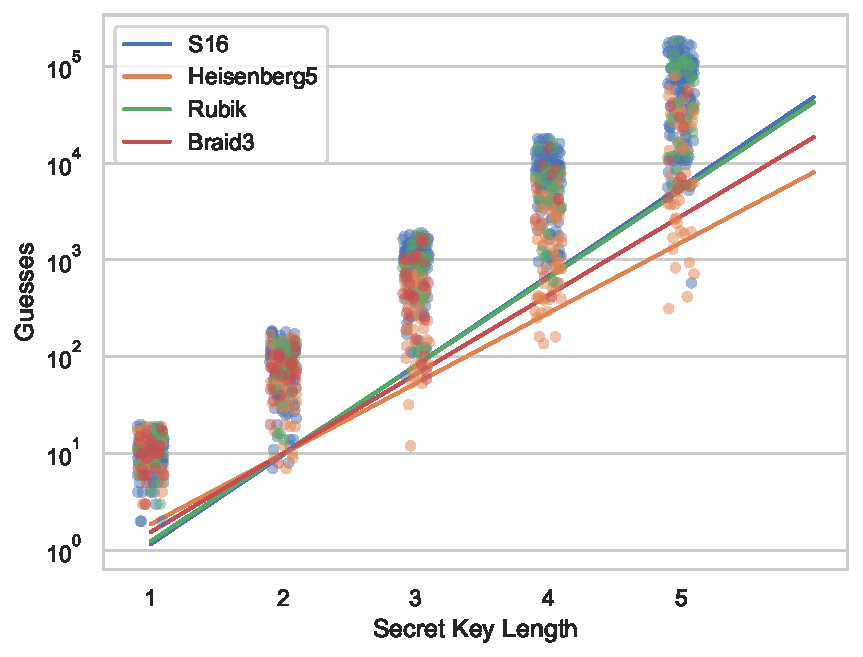
\includegraphics[width=\columnwidth]{images/Guesses-L.pdf}
  \caption{Comparison between groups with respect to number of guesses needed to obtain the shared key using the brute-force algorithm. Each group's performance is measured for various private key lengths, with public set size fixed at 5.}
  \label{fig:guess-l}
\end{figure}

\subsubsection{Relative Lengths}\label{sec:eval-relative-lengths}

Preliminary analysis showed that the average proportion of guesses made by the brute-force algorithm before it found a key \textit{decreases} as we increase the number of private key factors ($L$), for a fixed public key size ($N$). To investigate this, we hold fixed the size of the search space, and vary the values (namely, $L$ and $N$) that determine this size. The naive search space is size $(2N)^L$, so we must choose $N_1 \neq N_2$ and $L_1 \neq L_2$ satisfying the equality $(2N_1)^{L_1} = (2N_2)^{L_2}$. In Figure \ref{fig:fix-keyspace}, we use $(2 \cdot 2)^{2 L_2} = (2 \cdot 8)^{L_2}$, for $L_2 = 2, 3, ..., 7$.

\begin{figure}[hbt]
  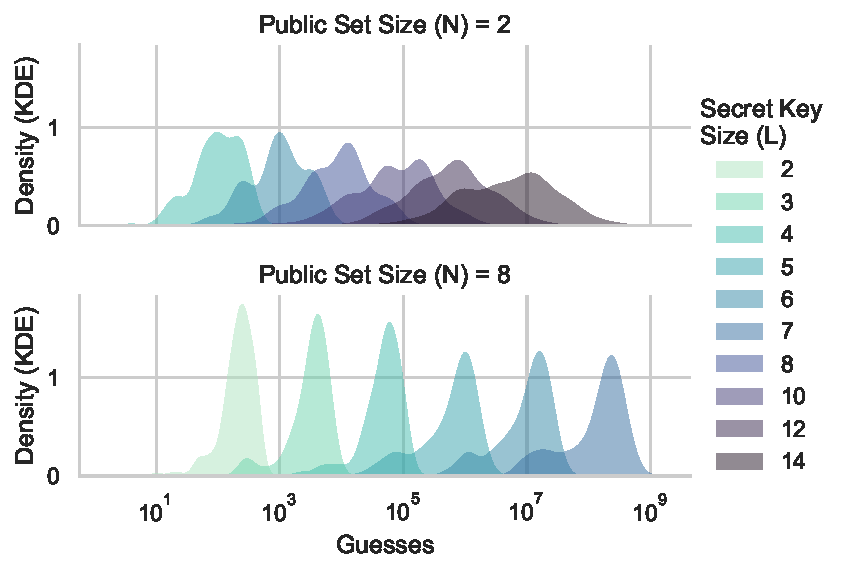
\includegraphics[width=\columnwidth]{images/constant-key-space.pdf}
  \caption{Density of guesses needed to obtain the shared key using the brute-force algorithm, against private keys of $L$ factors. Search space is comparable between the upper and lower graphs, which show different public set sizes $N$ (see Section \ref{sec:eval-relative-lengths}). Platform: $S_{16}$; 100 samples per curve.}
  \label{fig:fix-keyspace}
\end{figure}

The results from this test corroborate the initial observation: on brute-force, the average number of iterations required is much (and more consistently) higher when $N$ is bigger than $L$, even for equally sized search spaces. Curves in the lower graph in Figure \ref{fig:fix-keyspace} showing the larger public set size are all right-leaning. Compare this to the curves in the upper graph showing the smaller public set size (with larger secret keys). The upper graph curves are less agressively right-leaning, meaning that it is easier to brute force longer secret keys chosen from small public sets than it is to brute force short secret keys chosen from larger sets. 

Looking solely at the growth of the naive search space would suggest that Alice and Bob, constrained by a finite cost per exchange, can maximize their security by using very long private keys. After all, private key size is exponentially related to the number of permutations, whereas public set size only reflects the base of the exponent. On the contrary, this result indicates that security is actually favorable when public set size exceeds the number of private key factors. Running an identical test using the Rubik's Cube group as platform yields the same confirmation.

We explain this result by analogy. Consider searching an undirected graph representing the key space of a specific group. It is possible that multiple permutations of group elements multiply to reach the same value, so some nodes in the graph may be more connected than others. The graph exists in $N$ dimensions, as we have ammended the AAG protocol\footnote{See Section \ref{sec:bg-protocol} and related footnote.}, prohibiting public sets from containing any two elements in the same dimension.

In this situation, private key size is analogous to search depth, and public set size relates to the breadth that must be explored. Maximizing one of these factors while holding the other small produces a less than maximal search boundary. If some nodes in the graph are much more connected than others, increasing search depth without increasing breadth only serves to increase the number of times that you visit these highly connected nodes. The presence of these over-represented nodes explains the behavior in Figure \ref{fig:fix-keyspace}. Likewise, having breadth without depth only makes a certain border set of the nodes possible as destinations, limiting key entropy.

The topology of this graph for a given $N$ and $L$ depends on the structure of the chosen platform group, as well as the constituent elements of the public set and private key.
\section{Conclusion}
\label{sec:conclusion}

We have presented a generic implementation of the AAG key exchange protocol that works with any platform group defined in SageMath, and a baseline brute-force attack that should be universally applicable. We have performed a basic comparison between platform groups using small key sizes, and discovered that public set size is more important than expected. We believe that this tool has utility for future cryptographic research investigating the security of the AAG protocol under different platform groups as well as implementing novel attacks against such groups.

\paragraph{Future Work} 

The scope of this work is limited to a simple analysis of naive brute force attacks using small key sizes. Key sizes considered here are much smaller than those that would be used cryptographically; studying feasable key lengths would require more processing power than we had access to.

\paragraph{Notes on Optimality and Security} All results presented here rely on SageMath's implementations of group-theoretic operations. Any extra time taken due to suboptimal implementation of such operations can be factored out as it will be present in all analysis of attacks against said group.

This implementation is proposed for research use only, and of course, is not intended a real-world cryptographic setting. In addition to the practical suboptimalities, no effort is made to make the implementation secure. 


\bibliographystyle{ACM-Reference-Format}
\bibliography{bib}

\end{document}
